
\begin{center}
	\tikzset{every picture/.style={line width=0.75pt}} %set default line width to 0.75pt        
	
	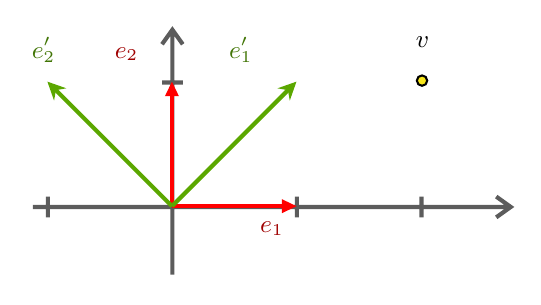
\begin{tikzpicture}[x=0.75pt,y=0.75pt,yscale=-1,xscale=1]
		%uncomment if require: \path (0,300); %set diagram left start at 0, and has height of 300
		
		%Shape: Axis 2D [id:dp342570794536994] 
		\draw [color={rgb, 255:red, 92; green, 92; blue, 92 }  ,draw opacity=1 ][line width=1.5]  (113,200.38) -- (343.25,200.38)(180.22,115) -- (180.22,233) (336.25,195.38) -- (343.25,200.38) -- (336.25,205.38) (175.22,122) -- (180.22,115) -- (185.22,122) (240.22,195.38) -- (240.22,205.38)(300.22,195.38) -- (300.22,205.38)(120.22,195.38) -- (120.22,205.38)(175.22,140.38) -- (185.22,140.38) ;
		\draw   ;
		%Straight Lines [id:da1818651961566673] 
		\draw [color={rgb, 255:red, 255; green, 0; blue, 0 }  ,draw opacity=1 ][line width=1.5]    (180,200) -- (236,200) ;
		\draw [shift={(240,200)}, rotate = 180] [fill={rgb, 255:red, 255; green, 0; blue, 0 }  ,fill opacity=1 ][line width=0.08]  [draw opacity=0] (6.97,-3.35) -- (0,0) -- (6.97,3.35) -- cycle    ;
		%Straight Lines [id:da6840376030942996] 
		\draw [color={rgb, 255:red, 255; green, 0; blue, 0 }  ,draw opacity=1 ][line width=1.5]    (180,200) -- (180,144) ;
		\draw [shift={(180,140)}, rotate = 90] [fill={rgb, 255:red, 255; green, 0; blue, 0 }  ,fill opacity=1 ][line width=0.08]  [draw opacity=0] (6.97,-3.35) -- (0,0) -- (6.97,3.35) -- cycle    ;
		%Straight Lines [id:da23828819589743078] 
		\draw [color={rgb, 255:red, 91; green, 167; blue, 0 }  ,draw opacity=1 ][line width=1.5]    (180,200) -- (237.17,142.83) ;
		\draw [shift={(240,140)}, rotate = 135] [fill={rgb, 255:red, 91; green, 167; blue, 0 }  ,fill opacity=1 ][line width=0.08]  [draw opacity=0] (8.75,-4.2) -- (0,0) -- (8.75,4.2) -- (5.81,0) -- cycle    ;
		%Straight Lines [id:da644259291625594] 
		\draw [color={rgb, 255:red, 91; green, 167; blue, 0 }  ,draw opacity=1 ][line width=1.5]    (180,200) -- (122.83,142.83) ;
		\draw [shift={(120,140)}, rotate = 45] [fill={rgb, 255:red, 91; green, 167; blue, 0 }  ,fill opacity=1 ][line width=0.08]  [draw opacity=0] (8.75,-4.2) -- (0,0) -- (8.75,4.2) -- (5.81,0) -- cycle    ;
		%Shape: Circle [id:dp8467208402612376] 
		\draw  [color={rgb, 255:red, 0; green, 0; blue, 0 }  ,draw opacity=1 ][fill={rgb, 255:red, 248; green, 231; blue, 28 }  ,fill opacity=1 ] (298,139.5) .. controls (298,138.12) and (299.12,137) .. (300.5,137) .. controls (301.88,137) and (303,138.12) .. (303,139.5) .. controls (303,140.88) and (301.88,142) .. (300.5,142) .. controls (299.12,142) and (298,140.88) .. (298,139.5) -- cycle ;
		
		% Text Node
		\draw (296,117) node [anchor=north west][inner sep=0.75pt]  [font=\small] [align=left] {$\displaystyle \ket{v}$};
		% Text Node
		\draw (221,206) node [anchor=north west][inner sep=0.75pt]  [font=\small,color={rgb, 255:red, 159; green, 0; blue, 0 }  ,opacity=1 ] [align=left] {$\displaystyle \ket{e_{1}}$};
		% Text Node
		\draw  [draw opacity=0]  (148,118) -- (182,118) -- (182,143) -- (148,143) -- cycle  ;
		\draw (151,122) node [anchor=north west][inner sep=0.75pt]  [font=\small,color={rgb, 255:red, 159; green, 0; blue, 0 }  ,opacity=1 ] [align=left] {$\displaystyle \ket{e_{2}}$};
		% Text Node
		\draw (206,117) node [anchor=north west][inner sep=0.75pt]  [font=\small,color={rgb, 255:red, 65; green, 117; blue, 5 }  ,opacity=1 ] [align=left] {$\displaystyle \ket{e'_{1}}$};
		% Text Node
		\draw (111,117) node [anchor=north west][inner sep=0.75pt]  [font=\small,color={rgb, 255:red, 65; green, 117; blue, 5 }  ,opacity=1 ] [align=left] {$\displaystyle \ket{e'_{2}}$};
		
	\end{tikzpicture}


\end{center}

	